\chapter{Quadrifilare Helixantenne (QFH)}
\label{chap:qfh}
Die Quadrifilare Helixantenne ist eine Abwandlung der monofilaren Helixantenne und unterscheidet sich von dieser in mehreren wichtigen Punkten.

Zum einen ist sie um einiges kleiner als die monofilare Helix. Zum anderen wird sie als omnidirektionale Antenne für Satellitenkommunikation verwendet, da sie, wie die monofilare Helixantenne, zirkular polarisiert ist. Sie zeigt entlang des Horizonts sowie direkt nach oben einen besseren Antennengewinn als in andere Richtungen.

\section{Design}
Das Design der QFH muss einigen Anforderungen entsprechen. Neben den Anforderungen die eigentliche Funktion zu erfüllen, scilicet für eine Frequenz von 433 Megahertz ein möglichst quasi-isotropes Abstrahlverhalten nach oben aufzuweisen und auf 50 Ohm angepasst zu sein, den Anforderungen durch die Natur gerecht zu werden. Dabei wird ein besonderes Augenmerk auf die UV-Resistenz und den Korrosionsschutz gelegt. 

Um Richtwerte für die Dimensionen einer QFH im 70cm-Band zu erhalten, wurde das Online-Tool unter \url{https://jcoppens.com/ant/qfh/calc.en.php} zur Dimensionierung von Antennen eingesetzt. Es ergeben sich dadurch folgende Werte:

\begin{center}
	\begin{tabular}{|c|c|c|}
		\hline
		\textbf{Parameter} & \textbf{kleine Schleife} & \textbf{große Schleife} \\
		\hline
		\textbf{Durchmesser} & 96.1 Millimeter & 101.1 Millimeter \\
		\hline
		\textbf{Höhe} & 218.4 Millimeter & 229.9 Millimeter \\
		\hline
	\end{tabular}
\end{center}

Mithilfe der Werte wurde folgendes 3D-Model der Antenne zur Simulation entworfen. Es gilt dabei zu erwähnen, dass, angetrieben von wissenschaftlicher Neugier, die QHA entgegen der typischen Konstruktion mit Kupferrohren aus Aluminiumstreifen und Aluminiumrundstäben simuliert und gefertigt wird. 

\begin{figure} [H]
	\centering
	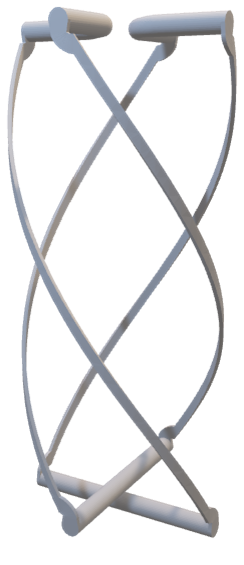
\includegraphics[width=.25\linewidth]{../ref/qfh_render.png}
	\caption{CAD-Model der QHA}
	\label{fig:qfh_render}
\end{figure}

Die Simulationsergebnisse der Antenne zeigen, dass sie bei einer Frequenz von 465 Megahertz die beste Performanz in Bezug auf die Anpassung besitzt. Bei dieser Frequenz erreicht sie eine Rückflussdämpfung von etwas unter -16 Dezibel, was sich mit den Ergebnissen vieler Antennen dieser Bauart deckt \cite{noauthor_qfh_nodate} \cite{keller_quadrifilar_2015}.

\begin{figure} [H]
	\centering
	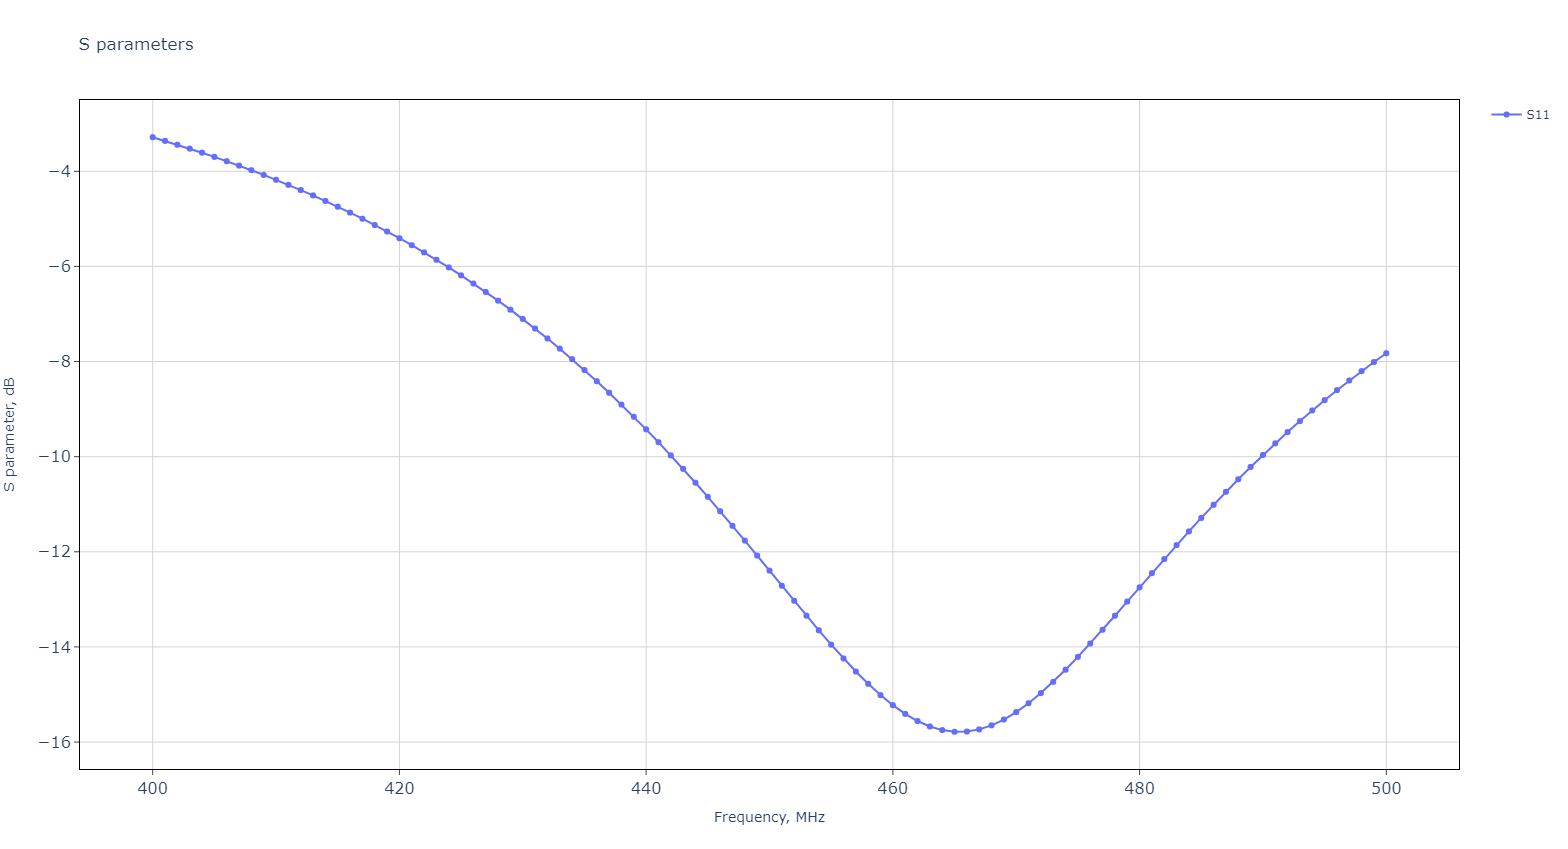
\includegraphics[width=\linewidth]{../ref/qfh_old_s11.png}
	\caption{S11-Parameter der ersten QFH}
	\label{fig:s11_old_qfh}
\end{figure}

Die Form des Abstrahlverhaltens sowie der maximale Gewinn mit 4.13 Dezibel entsprechen ebenfalls typischer Werte für eine QHA \cite{keller_quadrifilar_2015}.

\begin{figure} [H]
	\centering
	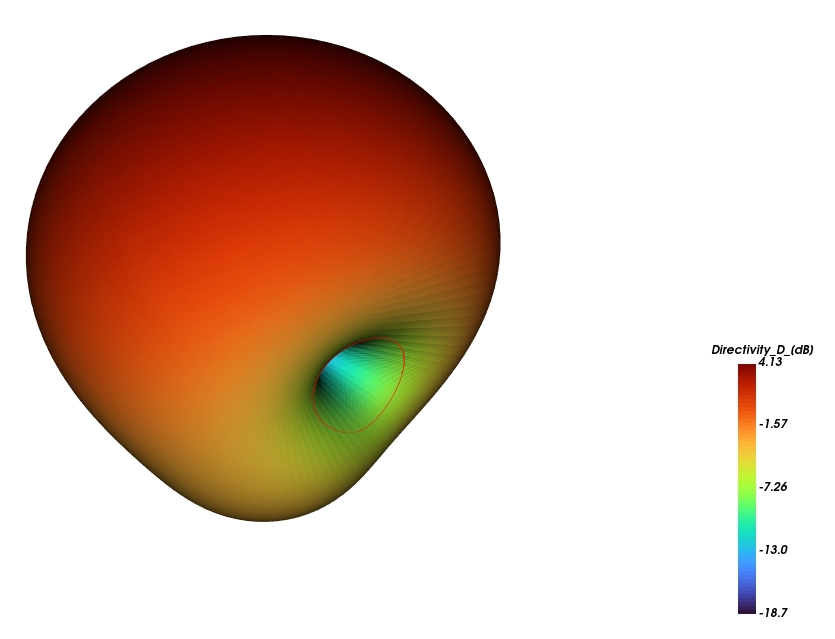
\includegraphics[width=.75\linewidth]{../ref/radiation_pattern_old_qfh.png}
	\caption{Abstrahlverhalten der ersten QHA bei 465 Megahertz}
	\label{fig:rp_old_qha}
\end{figure}

Durch gezielte Anpassung der Durchmesser und Längen einzelner Schleifen sowie zahlreicher Simulationen wurden mithilfe dieser Informationen Werte ermittelt, die eine optimale Leistung bei etwas unter den gewünschten 433 Megahertz erzielen. Eine leicht überdimensionierte Auslegung erleichtert die spätere Feinabstimmung, da es einfacher ist, Bauteile zu verkleinern, als sie zu vergrößern.

Daraus ergeben sich die folgenden finalen Werte:

\begin{center}
	\begin{tabular}{|c|c|c|}
		\hline
		\textbf{Parameter} & \textbf{kleine Schleife} & \textbf{große Schleife} \\
		\hline
		\textbf{Durchmesser} & 101.9 Millimeter & 107.1 Millimeter \\
		\hline
		\textbf{Höhe} & 231.7 Millimeter & 243.4 Millimeter \\
		\hline
	\end{tabular}
\end{center} 

Bei der Simulation dieser Werte ergibt sich eine Rückflussdämpfung von -13.7 Dezibel und ein maximaler Gewinn von 3.55 Dezibel bei 433 Megahertz. Die beste Anpassung besitzt die QHA bei 426 Megahertz mit einer Rückflussdämpfung von -14.4 Dezibel.

\begin{figure} [H]
	\centering
	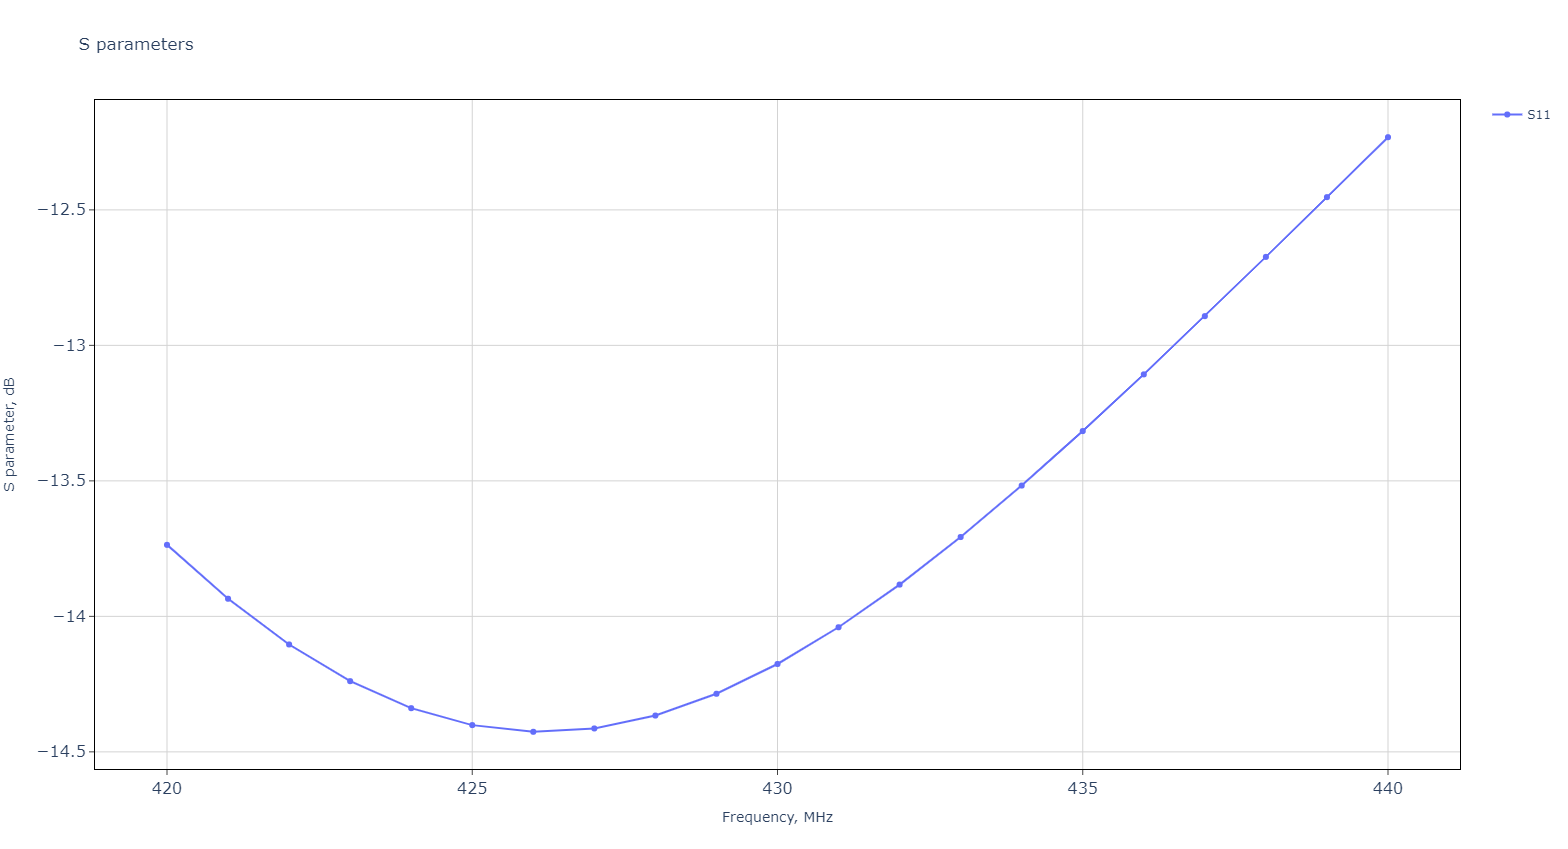
\includegraphics[width=\linewidth]{../ref/qfh_final_s11.png}
	\caption{S11-Parameter (Rückflussdämpfung) der finalen QHA}
	\label{fig:s11_final_qha}
\end{figure}

\begin{figure} [H]
	\centering
	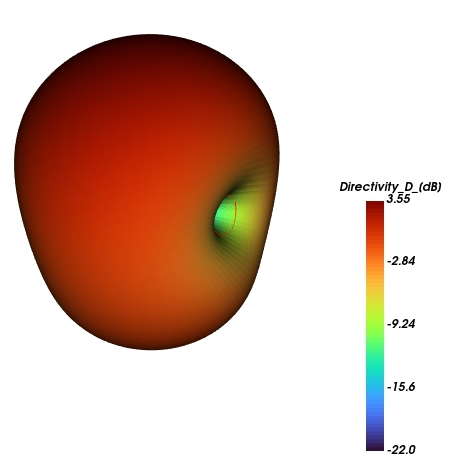
\includegraphics[width=.75\linewidth]{../ref/radiation_pattern_final_qfh.png}
	\caption{Abstrahlverhalten der finalen QHA bei 433 Megahertz}
	\label{fig:rp_final_qha}
\end{figure}

\section{Realisierung}
Für die Realisierung der Helixantenne werden folgende Materialien benötigt:\newline
- 4 Streifen mit 10x2 Millimeter Querschnitt aus Aluminiumblech für die Schleifen (jeweils mindestens 300 Millimeter lang)\newline
- 1x Aluminiumrundstab mit 10 Millimeter Durchmesser und 103.1 Millimeter Länge für den unteren Verbinder der großen Schleife\newline
- 1x Aluminiumrundstab mit 10 Millimeter Durchmesser und 97.9 Millimeter Länge für den unteren Verbinder der kleinen Schleife\newline
- 2x Aluminiumrundstab mit 10 Millimeter Durchmesser und 41.55 Millimeter Länge für den oberen Verbinder der großen Schleife\newline
- 2x Aluminiumrundstab mit 10 Millimeter Durchmesser und 38.95 Millimeter Länge für den oberen Verbinder der kleinen Schleife\newline
- 8x M4x10 Edelstahlsenkkopfschrauben zur Befestigung der Schleifen an den Verbindern\newline
- 4x M4x10 Messingschrauben als Lötpunkt für das Antennenkabel \newline
- 1x 400 Millimeter langes UV-beständiges PVC-Rohr mit 40 Millimeter Außendurchmesser und 3 Millimeter Wanddurchmesser.

Für das Biegen der Aluminiumstreifen wurden mithilfe eines 3D-Druckers Schablonen gefertigt um welche die Streifen gebogen werden können. 

\begin{figure} [H]
	\centering
	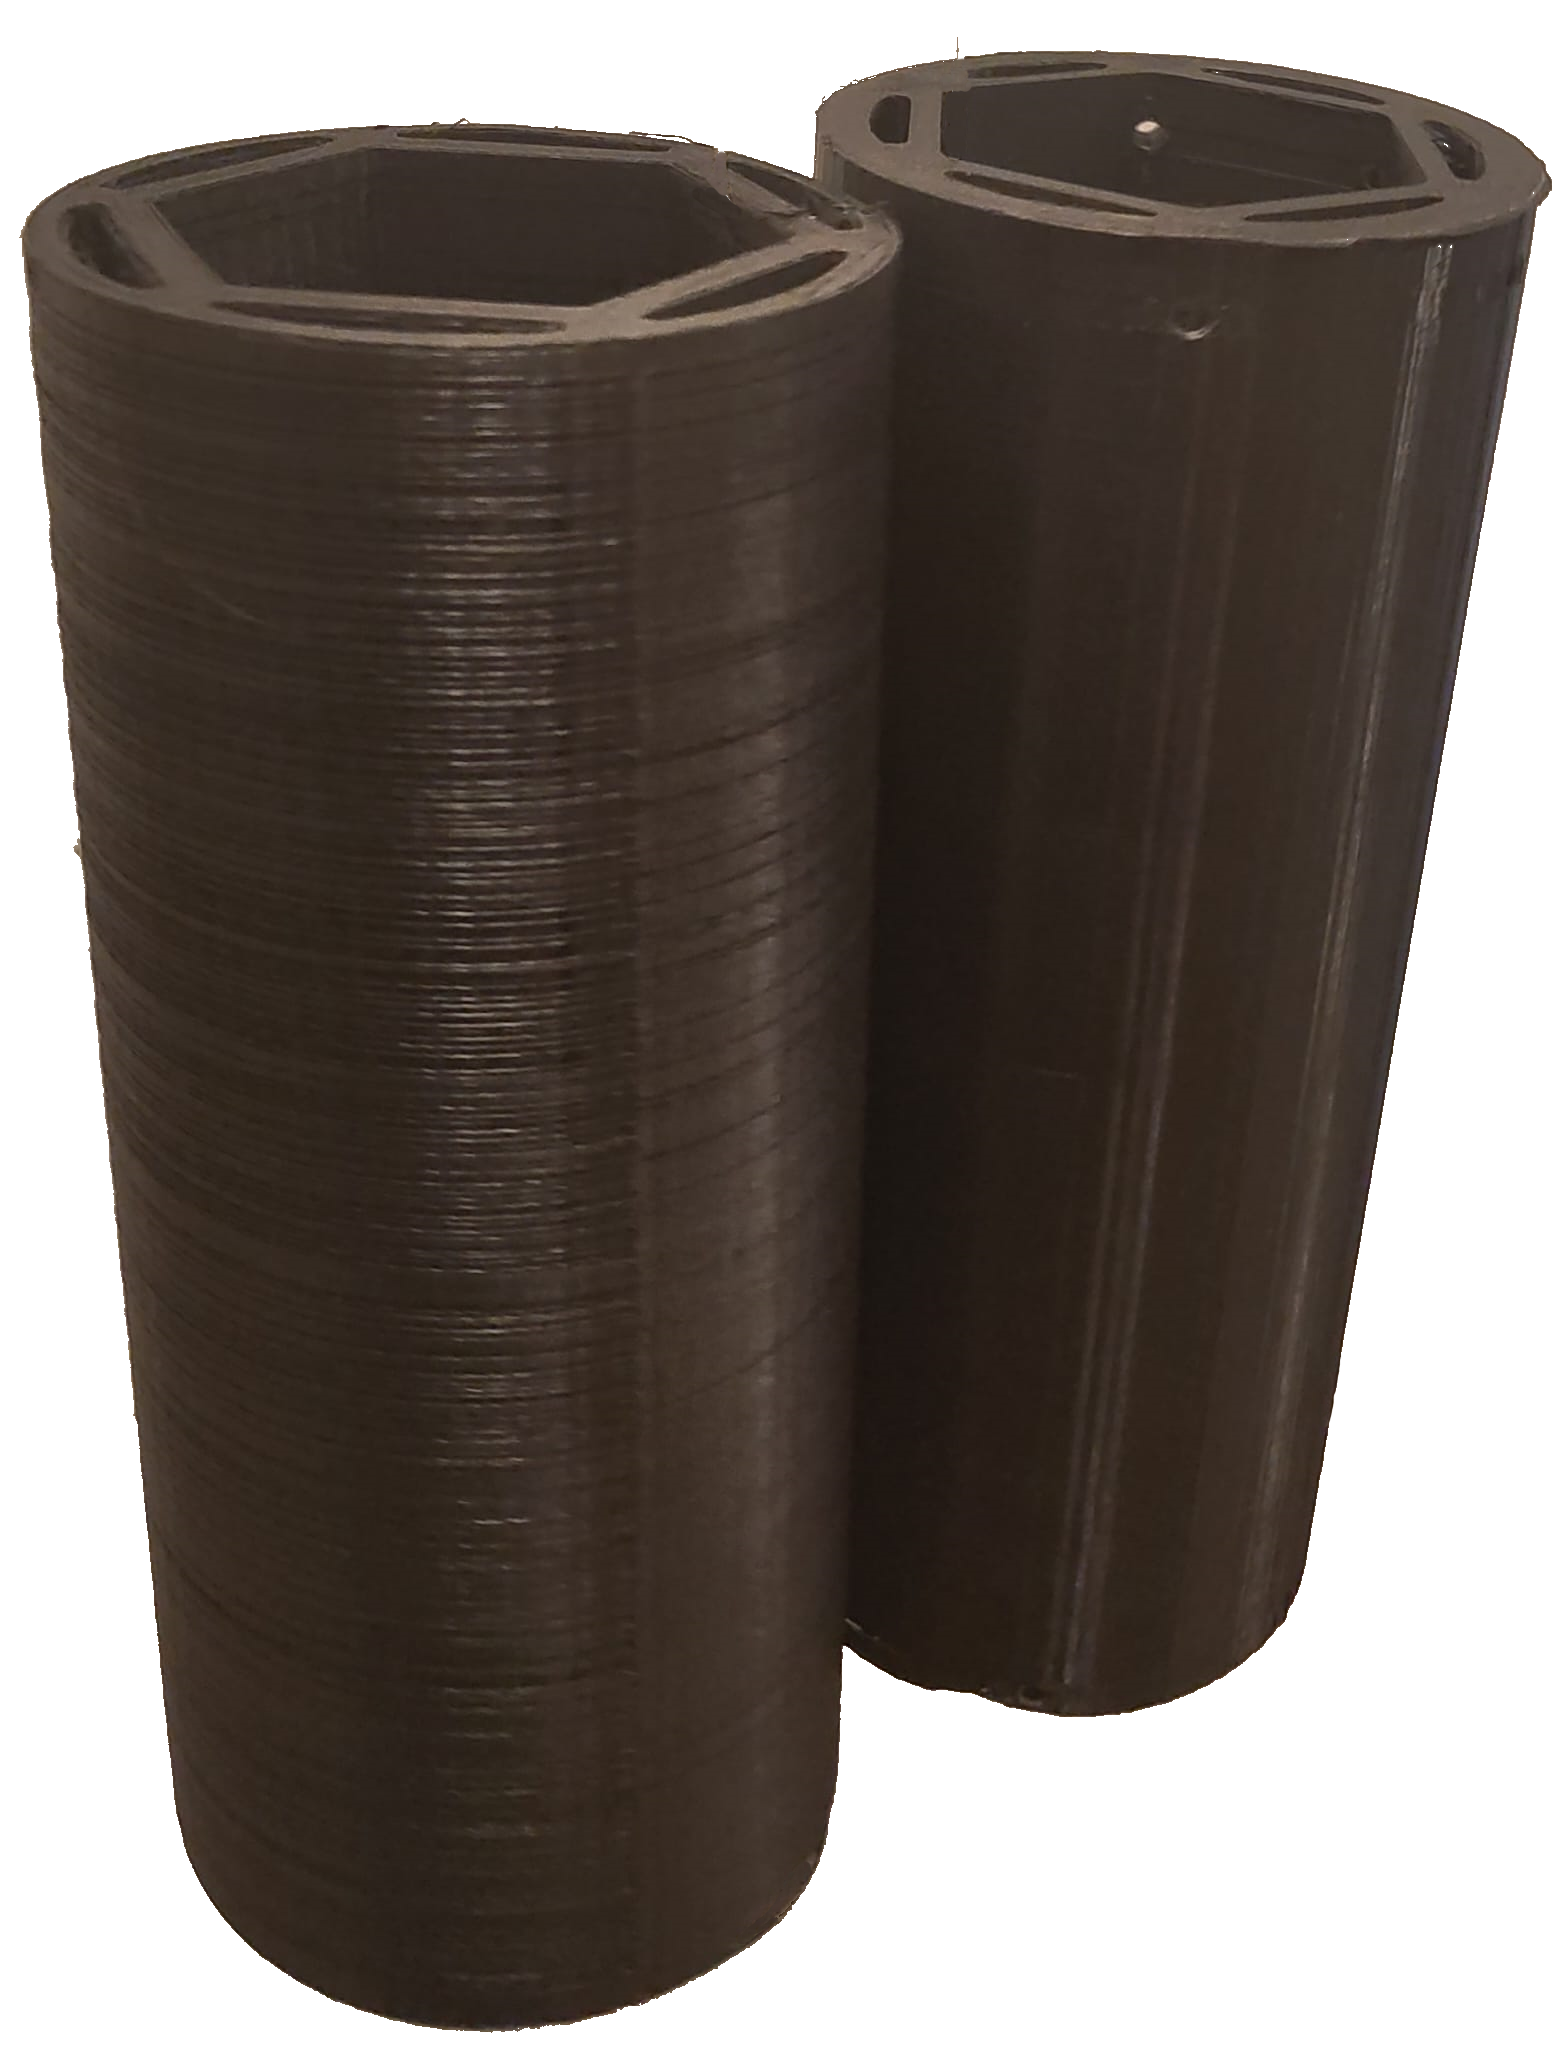
\includegraphics[width=.25\linewidth]{../ref/qfh_biegschablone.png}
	\caption{Biege-Schablonen für die Fertigung der kleinen und großen Schleifen}
	\label{fig:schablonen_qha}
\end{figure}

Die Aluminiumrundstäbe werden auf beiden Seiten mit einem M4-Gewinde versehen.

\begin{figure} [H]
	\centering
	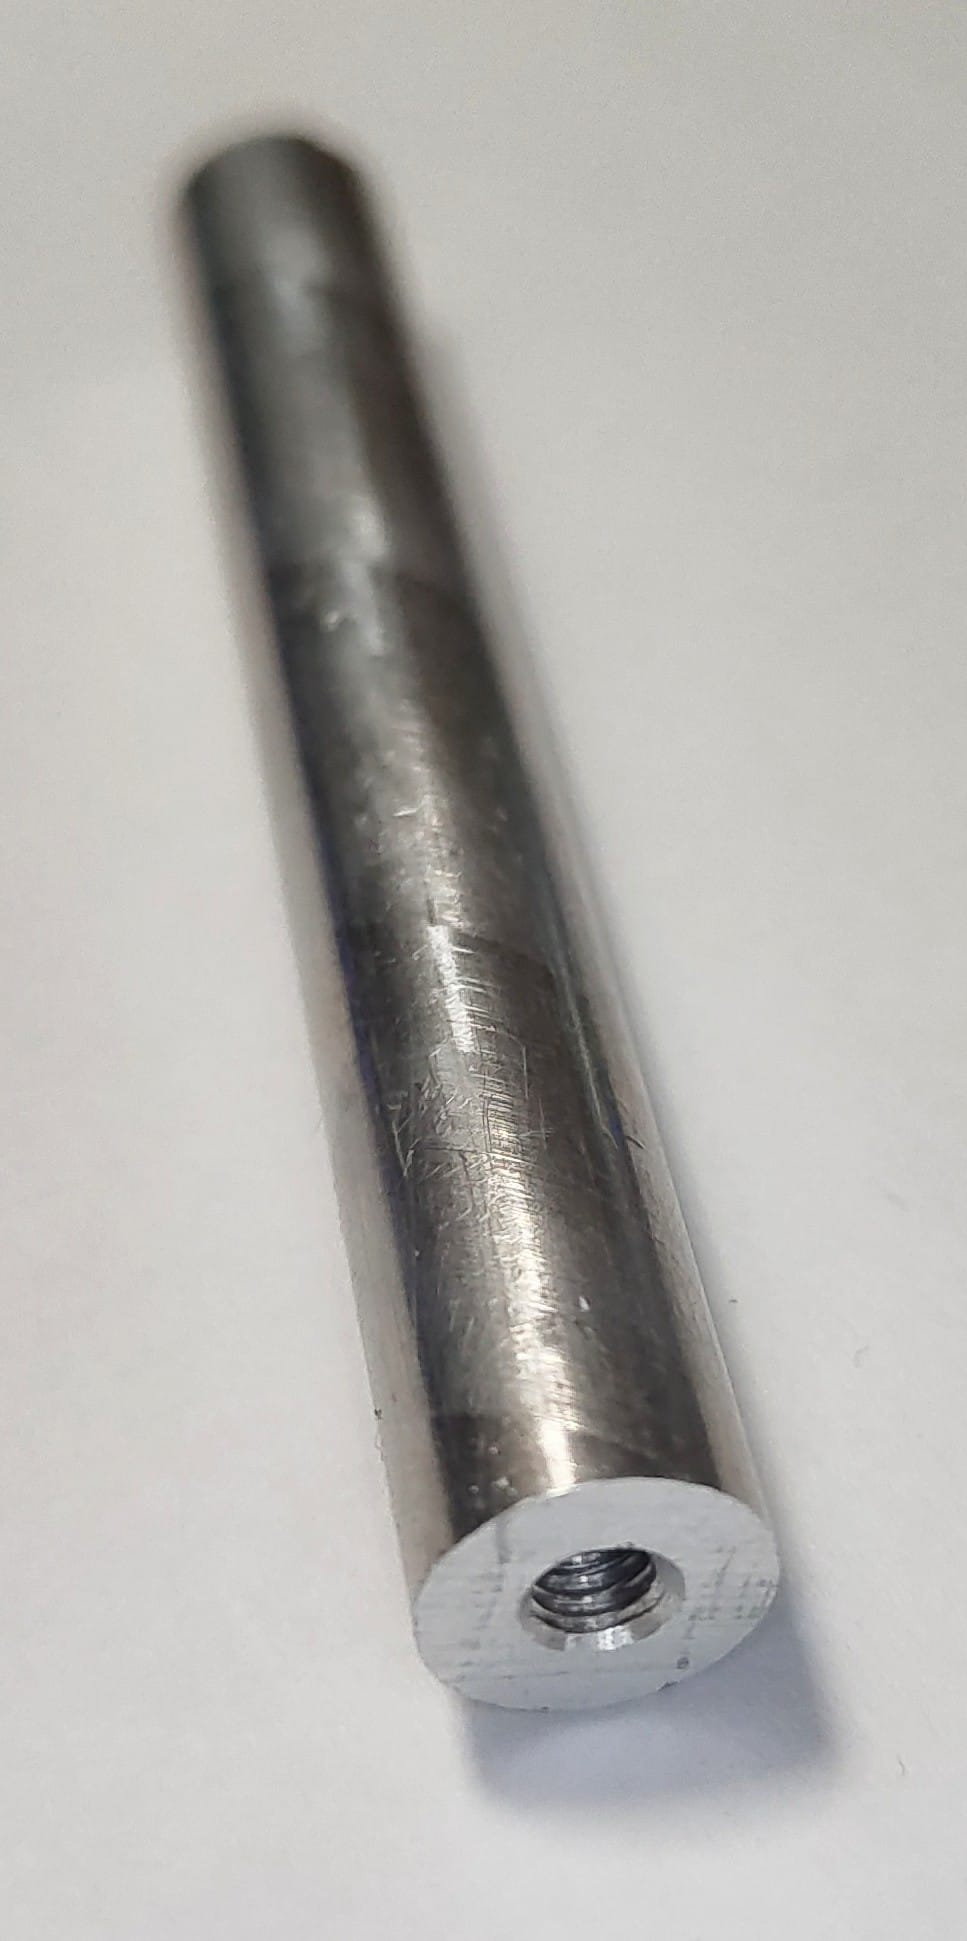
\includegraphics[width=.25\linewidth]{../ref/qfh_separator.jpeg}
	\caption{Beispiel eines fertigen Aluminiumrundstab}
	\label{fig:separator_qha}
\end{figure}

Die Aluminiumstäbe wurden mithilfe von 2-Komponenten Epoxidkleber in den gebohrten Löchern des PVC-Rohrs befestigt. Das Antennenkabel wurde entsprechend der nachfolgenden Abbildung an die Messingschrauben angelötet. 

\begin{figure} [H]
	\centering
	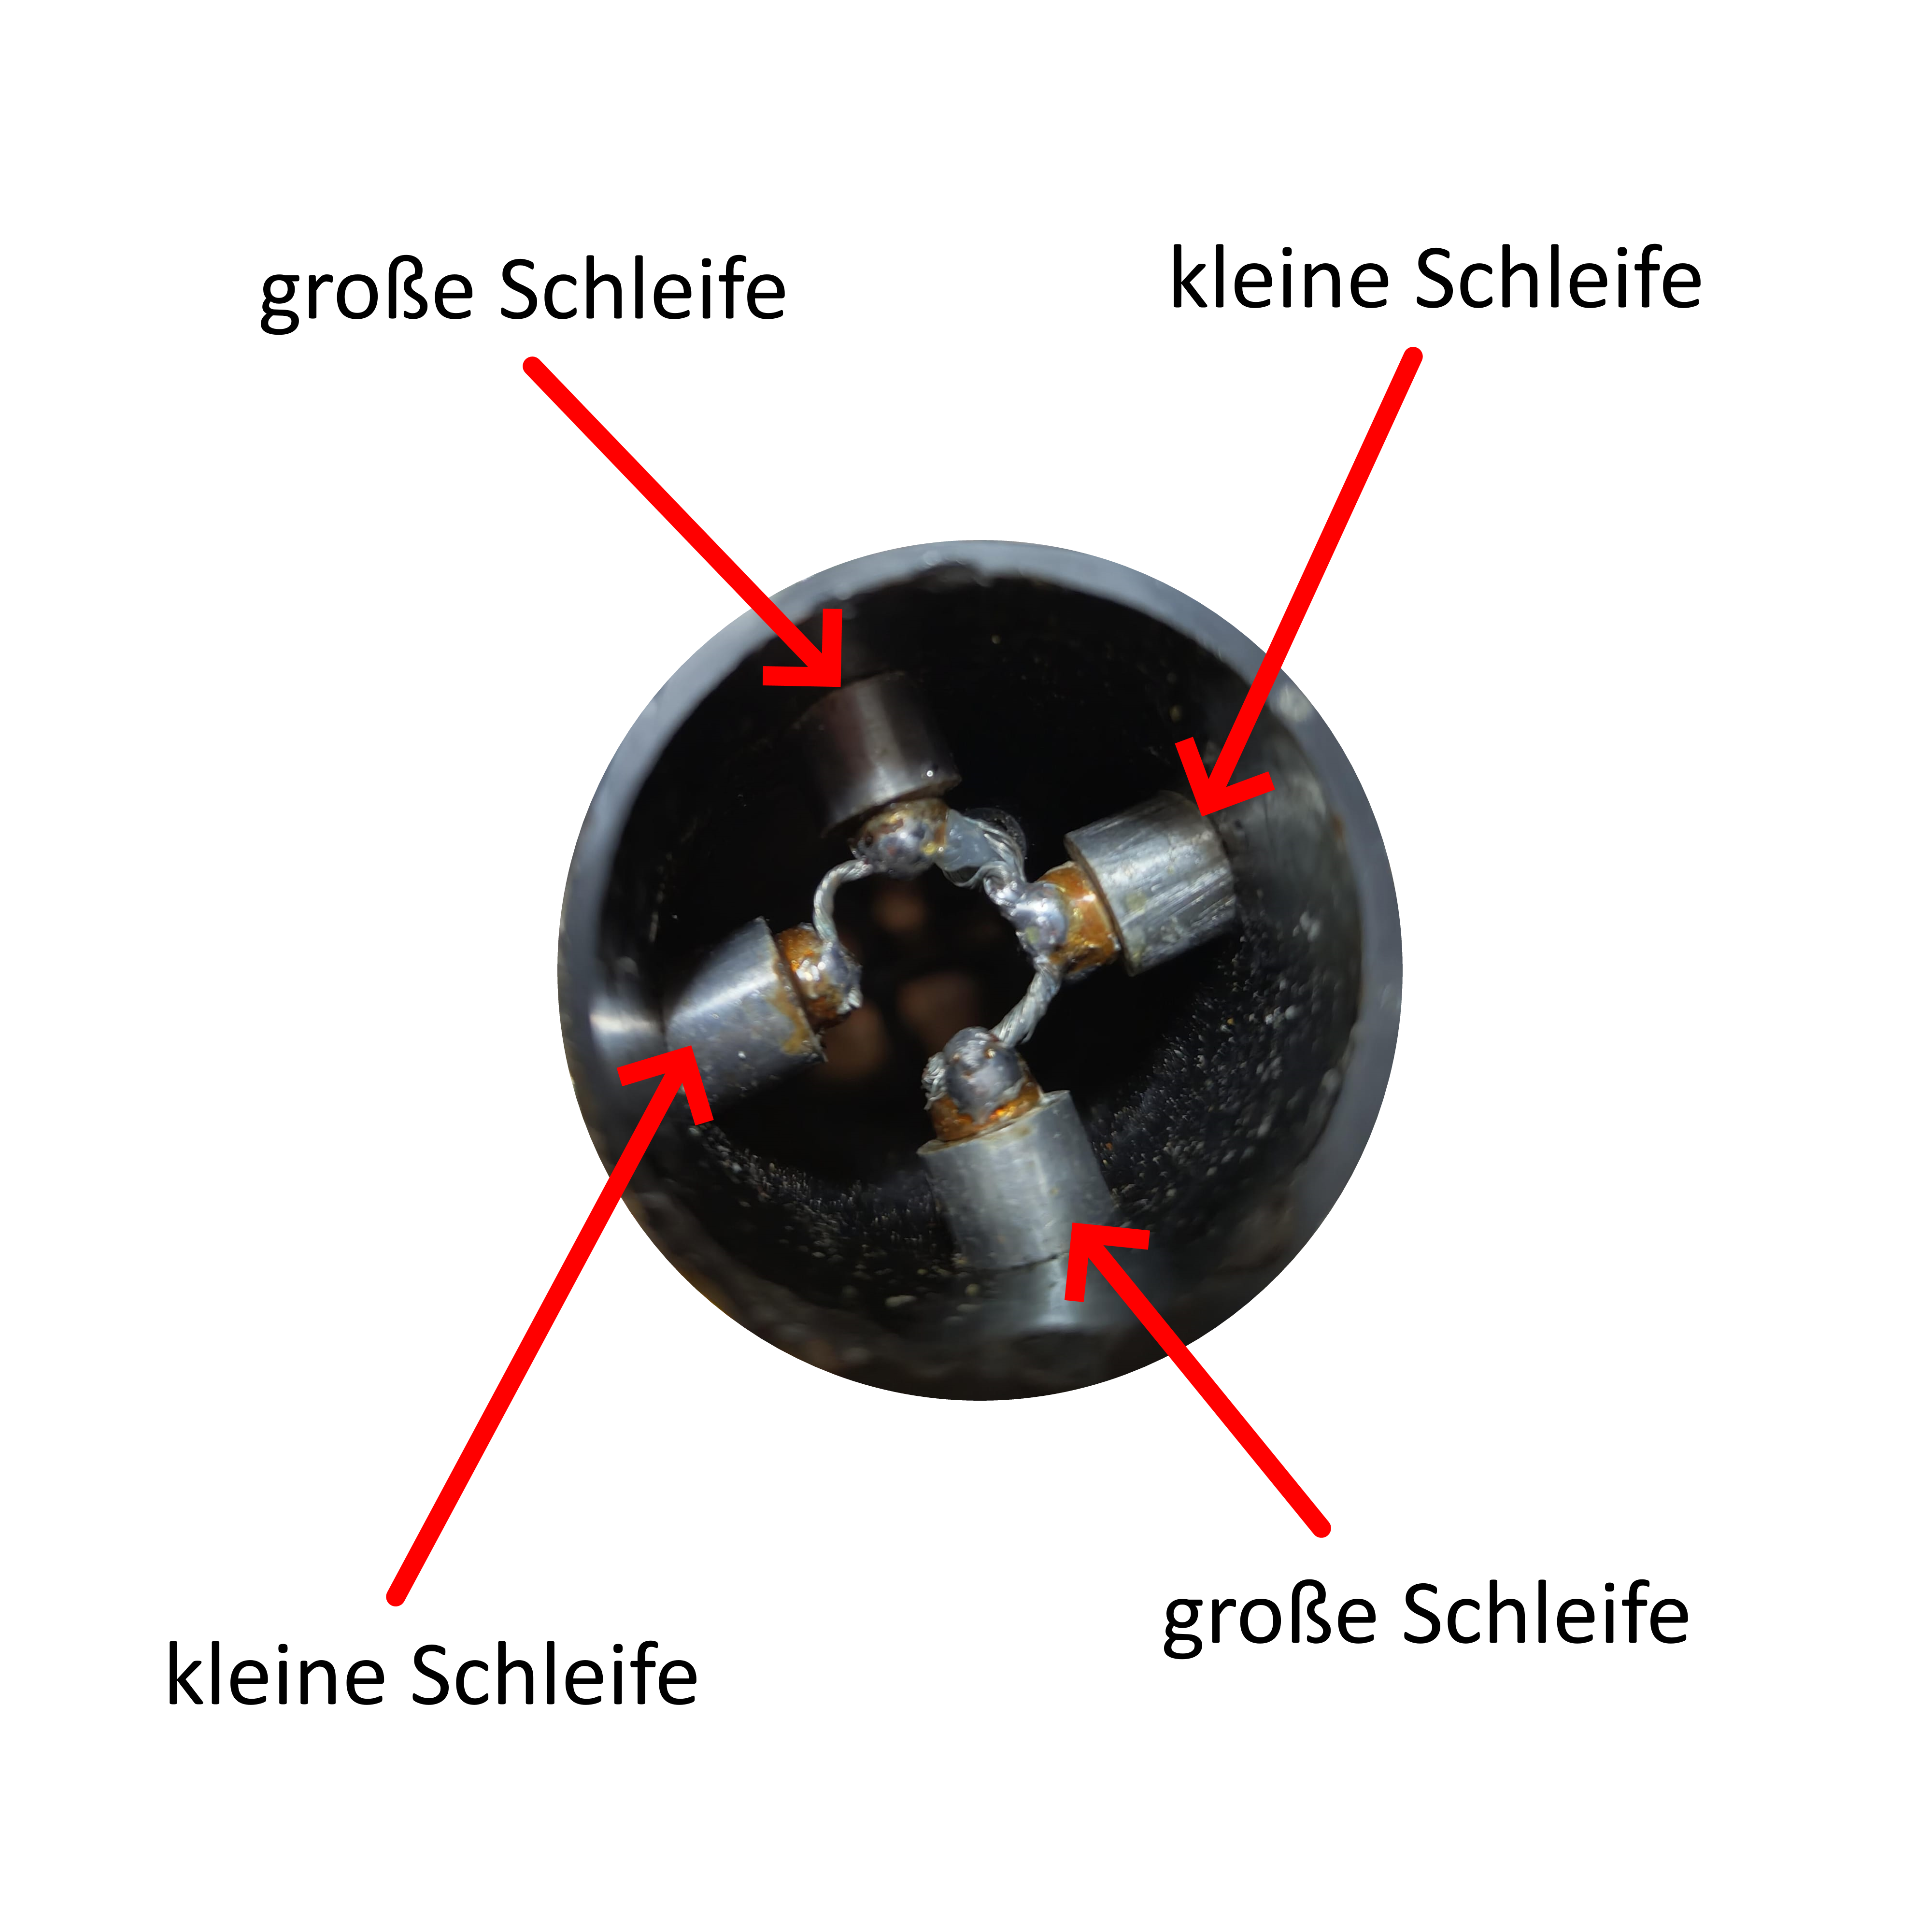
\includegraphics[width=.5\linewidth]{../ref/qfh_feedpoint.png}
	\caption{Anschluss des Antennenkabels an die QHA}
	\label{fig:feedpoint_qha}
\end{figure}

Vor eindringendem Regenwasser wird das Antennenkabel mithilfe eines 3D-gedrucktem Deckel für das PVC-Rohr geschützt. 

\begin{figure} [H]
	\centering
	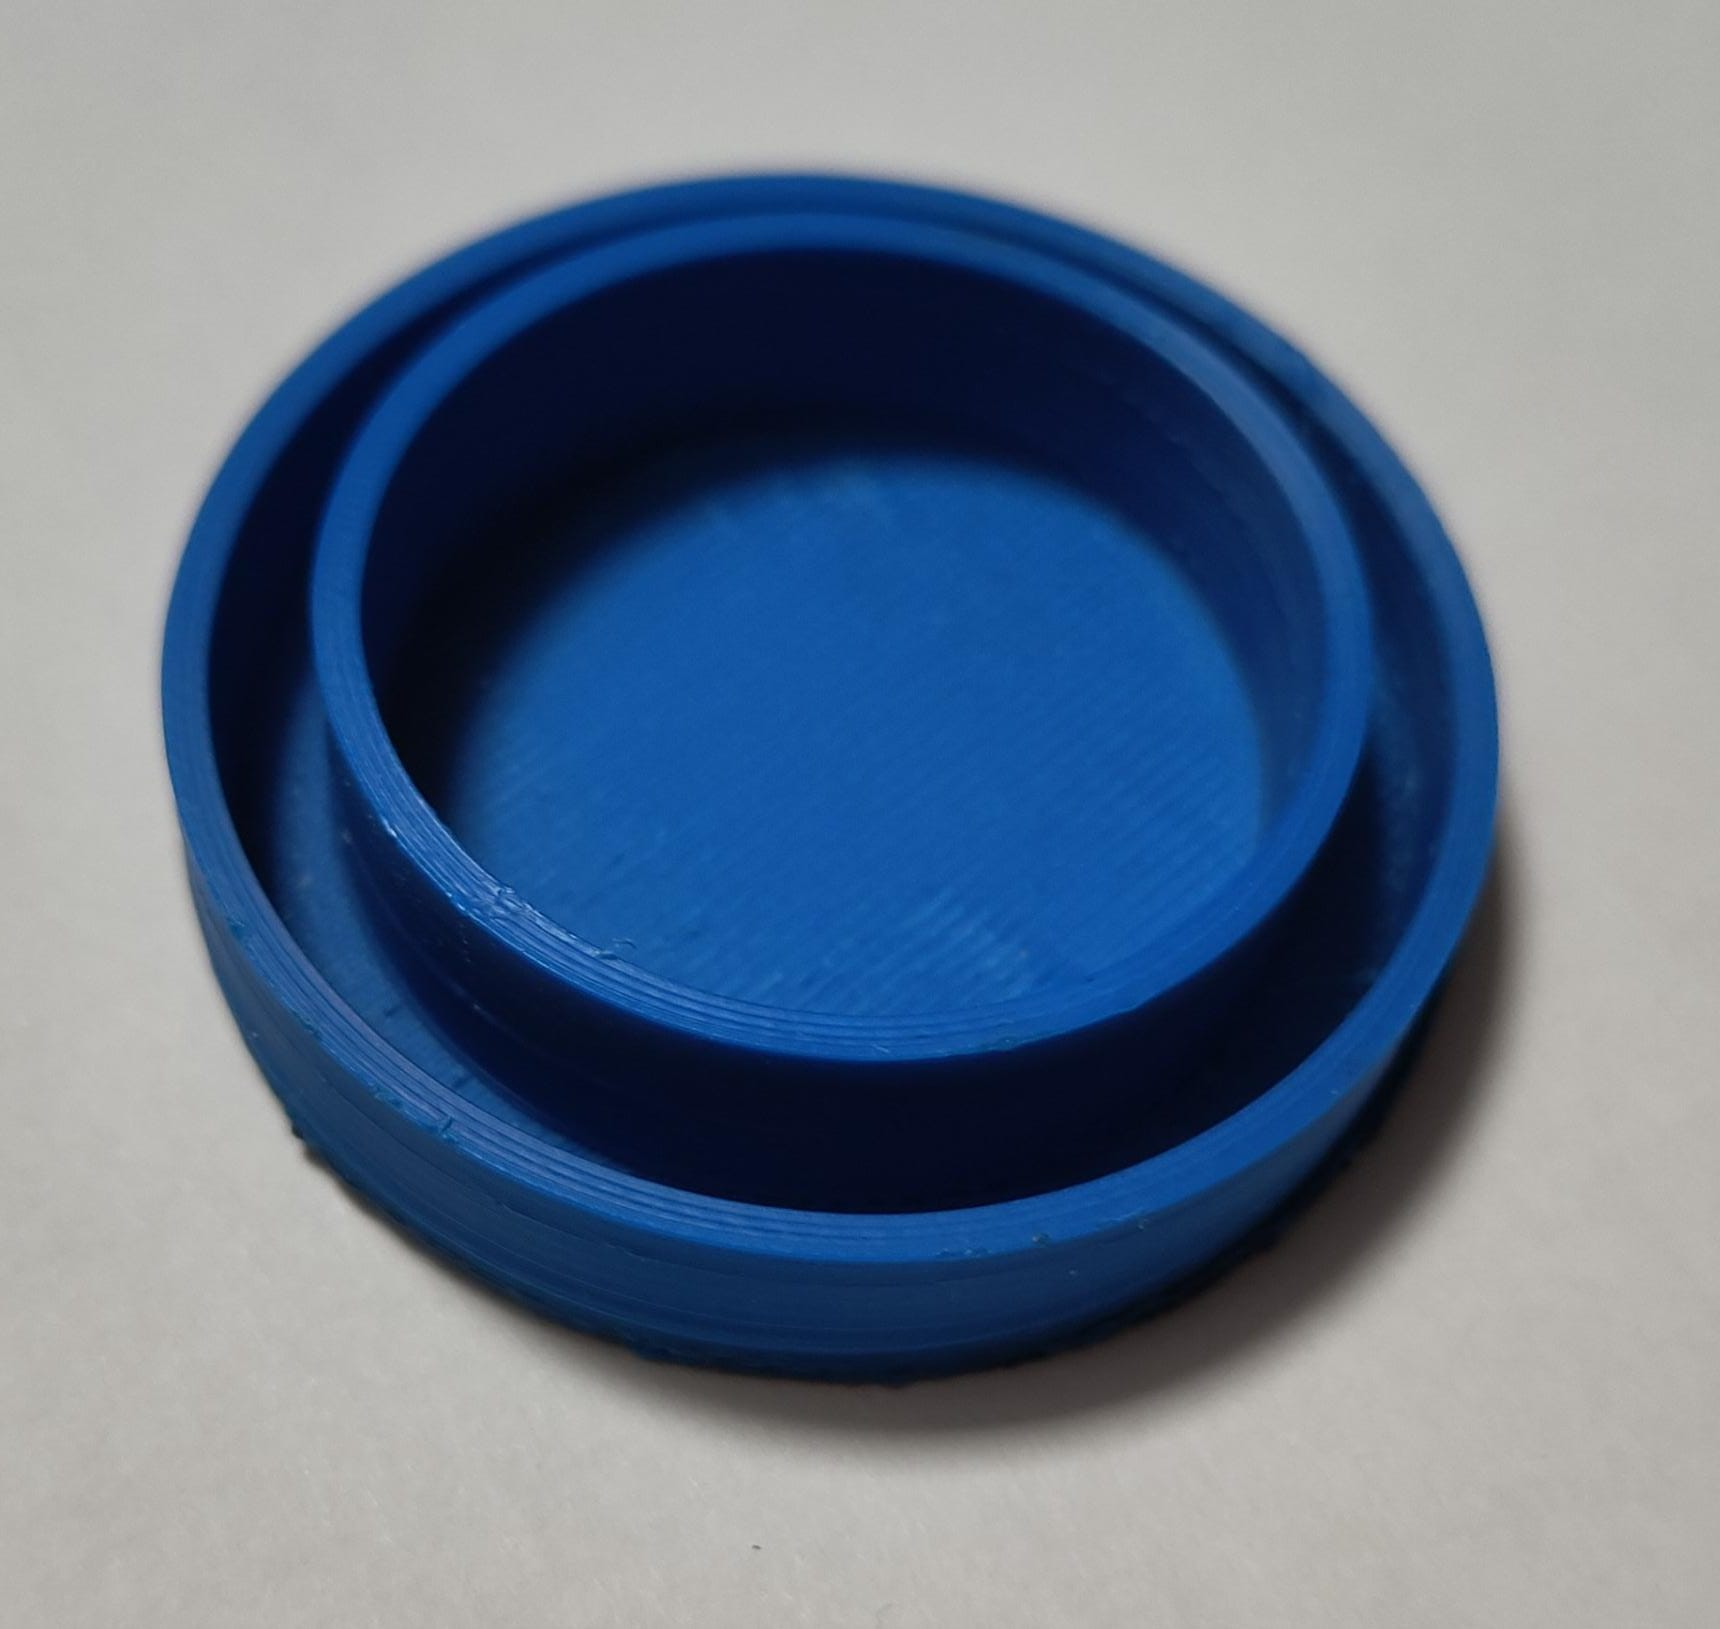
\includegraphics[width=.25\linewidth]{../ref/qfh_deckel.jpeg}
	\caption{Deckel für das PVC-Rohr}
	\label{fig:deckel_qha}
\end{figure}

Da die QHA eine symmetrische Antenne ist, weist die fertige QHA vier Wicklungen des Antennenkabels um das PVC-Rohr auf. Diese Art der Eliminierung von Mantelwellenströmen hat sich beim Bau von quadrifilaren Helixantennen etabliert \cite{noauthor_quadrifilar_nodate}. 

\begin{figure} [H]
	\centering
	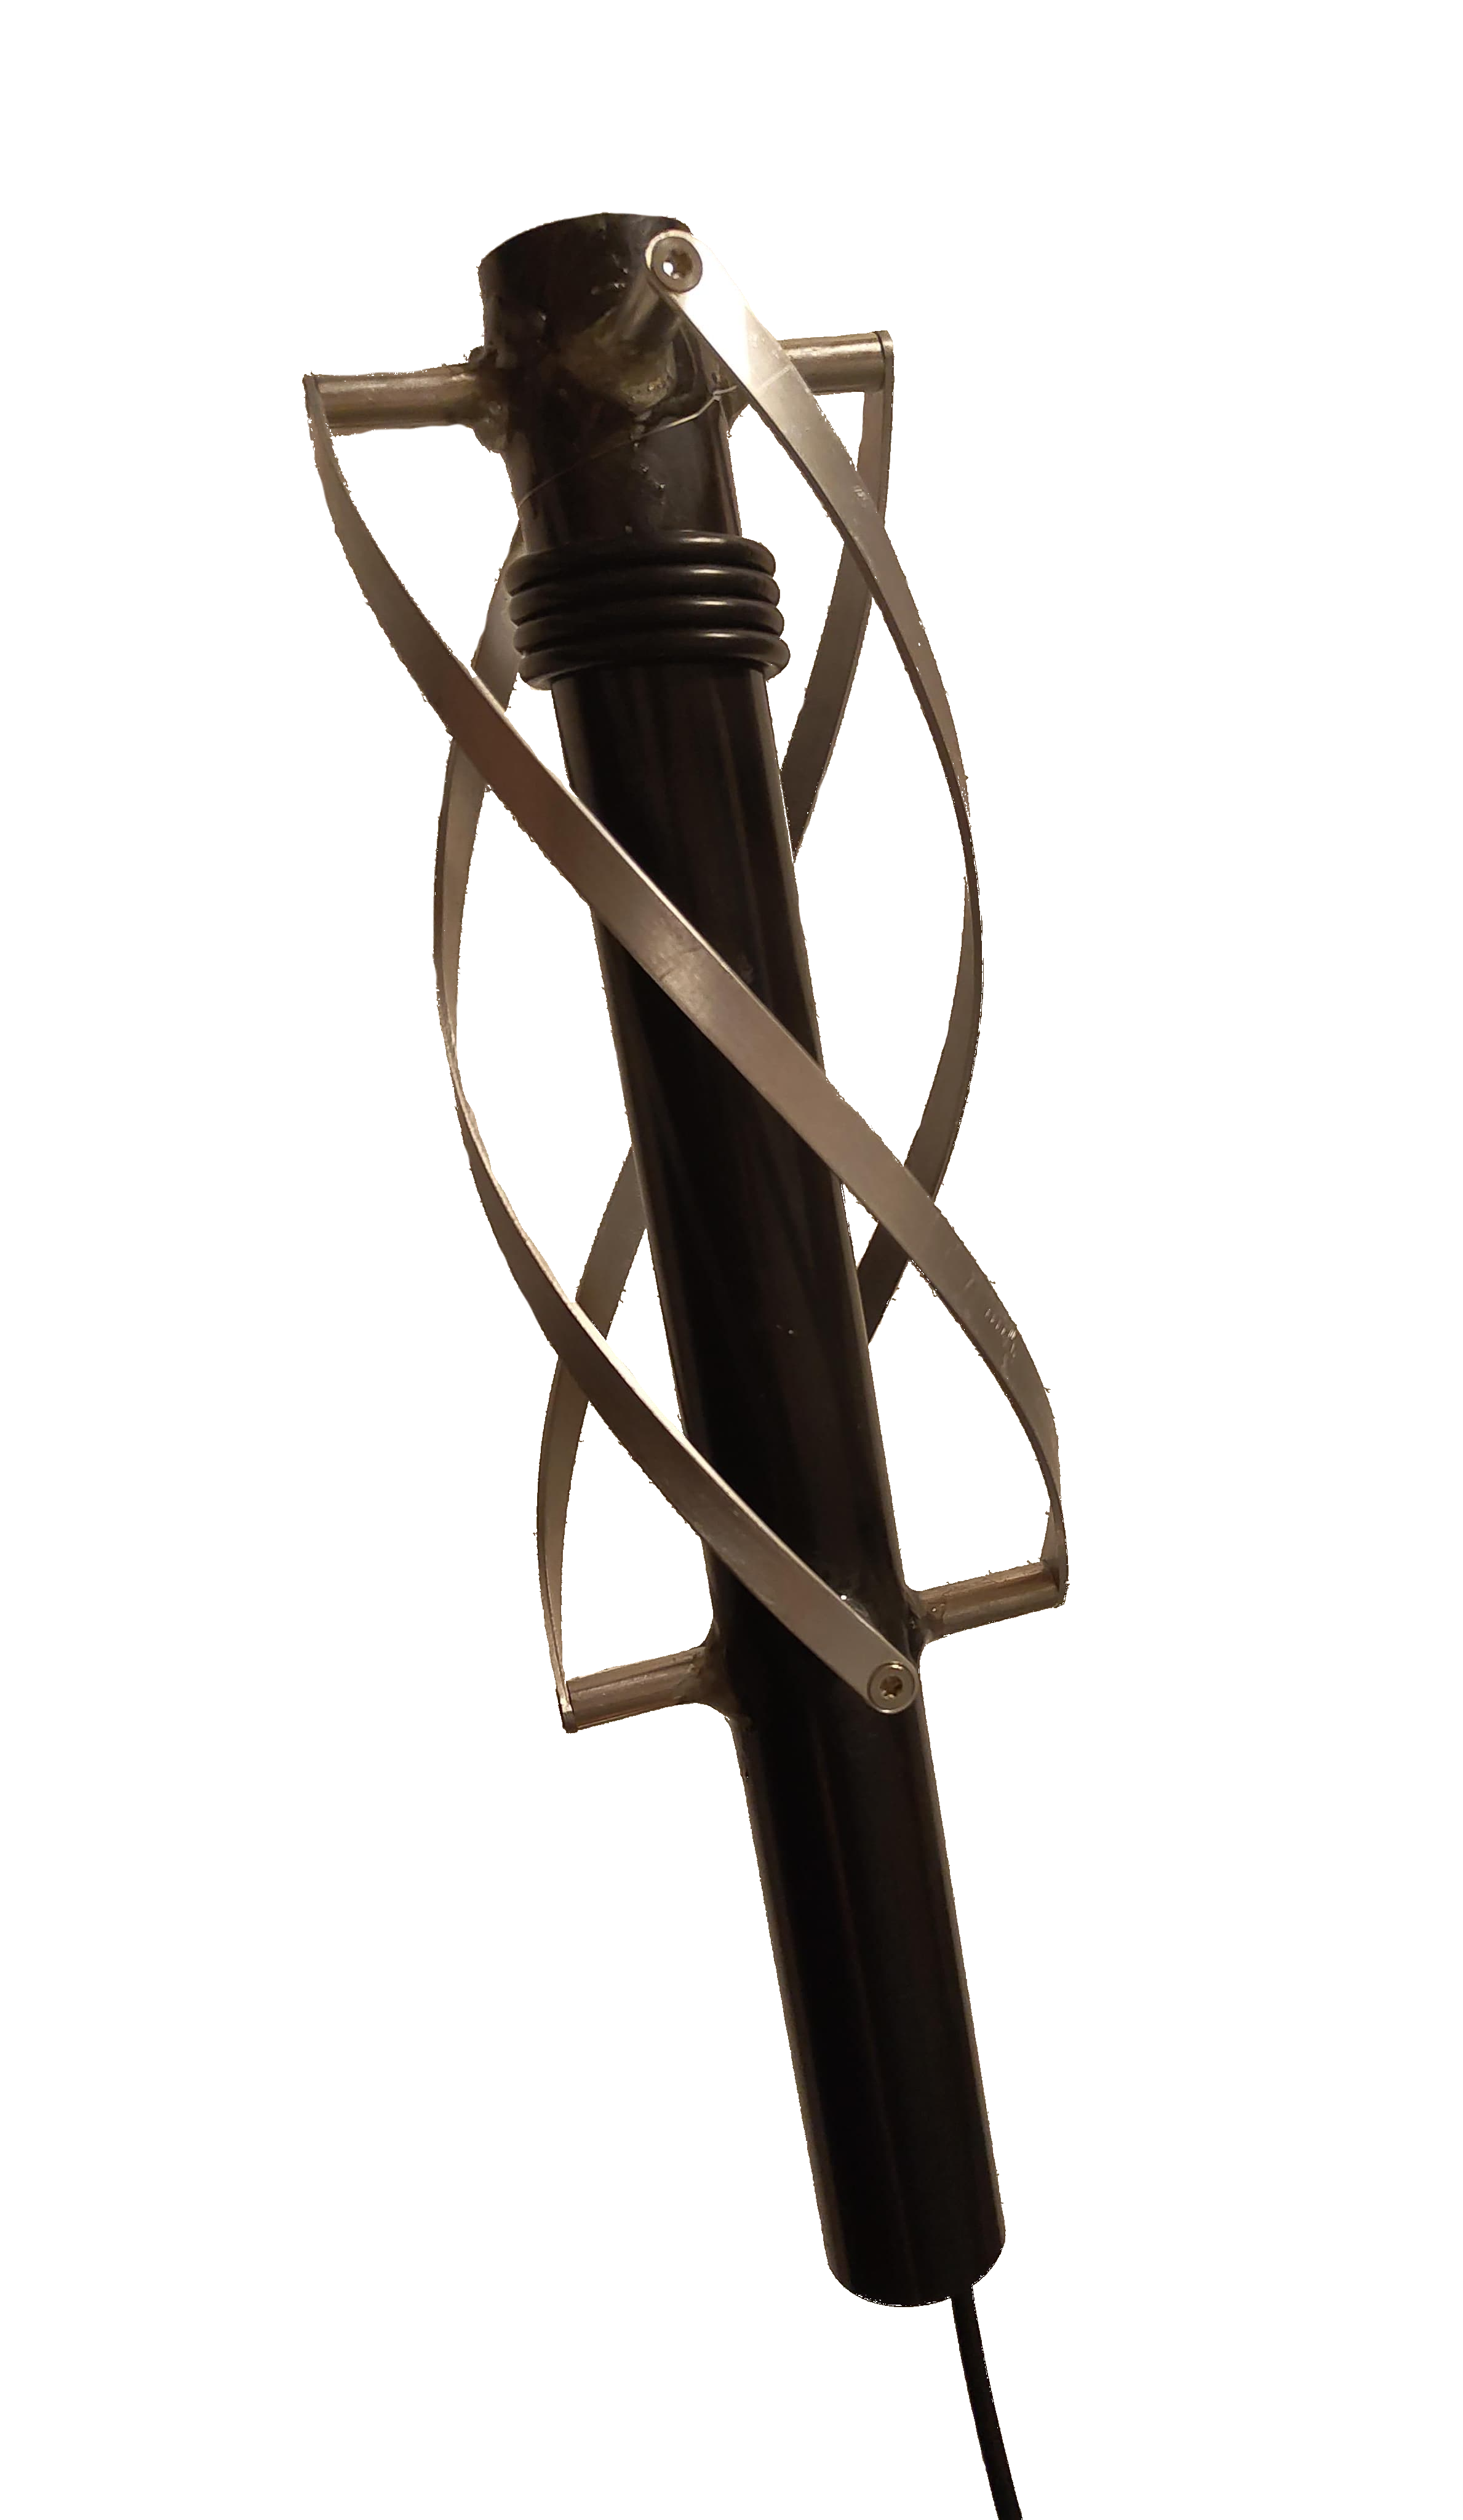
\includegraphics[width=.25\linewidth]{../ref/qha_fertig.png}
	\caption{Fertige QHA mit Mantelwellensperre}
	\label{fig:fertig_qha}
\end{figure}

Für die Anpassung der QHA relevant waren vorallem die Länge des abisolierten und nicht geschirmten Antennenkabels und die Form der Schleifen. Durch das minimieren der abisolierten Länge des Antennenkabels sowie das leichte korrigieren der Form der Schleifen konnte eine Rückflussdämpfung von -17.44 Dezibel bei einer Frequenz von 433 Megahertz erreicht werden, wie im nachfolgenden Kapitel (\ref{sec:messungen_qha}) zu sehen ist. Die Mantelwellensperre nahm keinen Einfluss auf die Anpassung und die Ergebnisse blieben mit und ohne Mantelwellensperre nahezu dieselben. 

\section{Messungen}
\label{sec:messungen_qha}
\subsection{Rückflussdämpfung und Smith-Diagramm}
\begin{figure} [H]
	\centering
	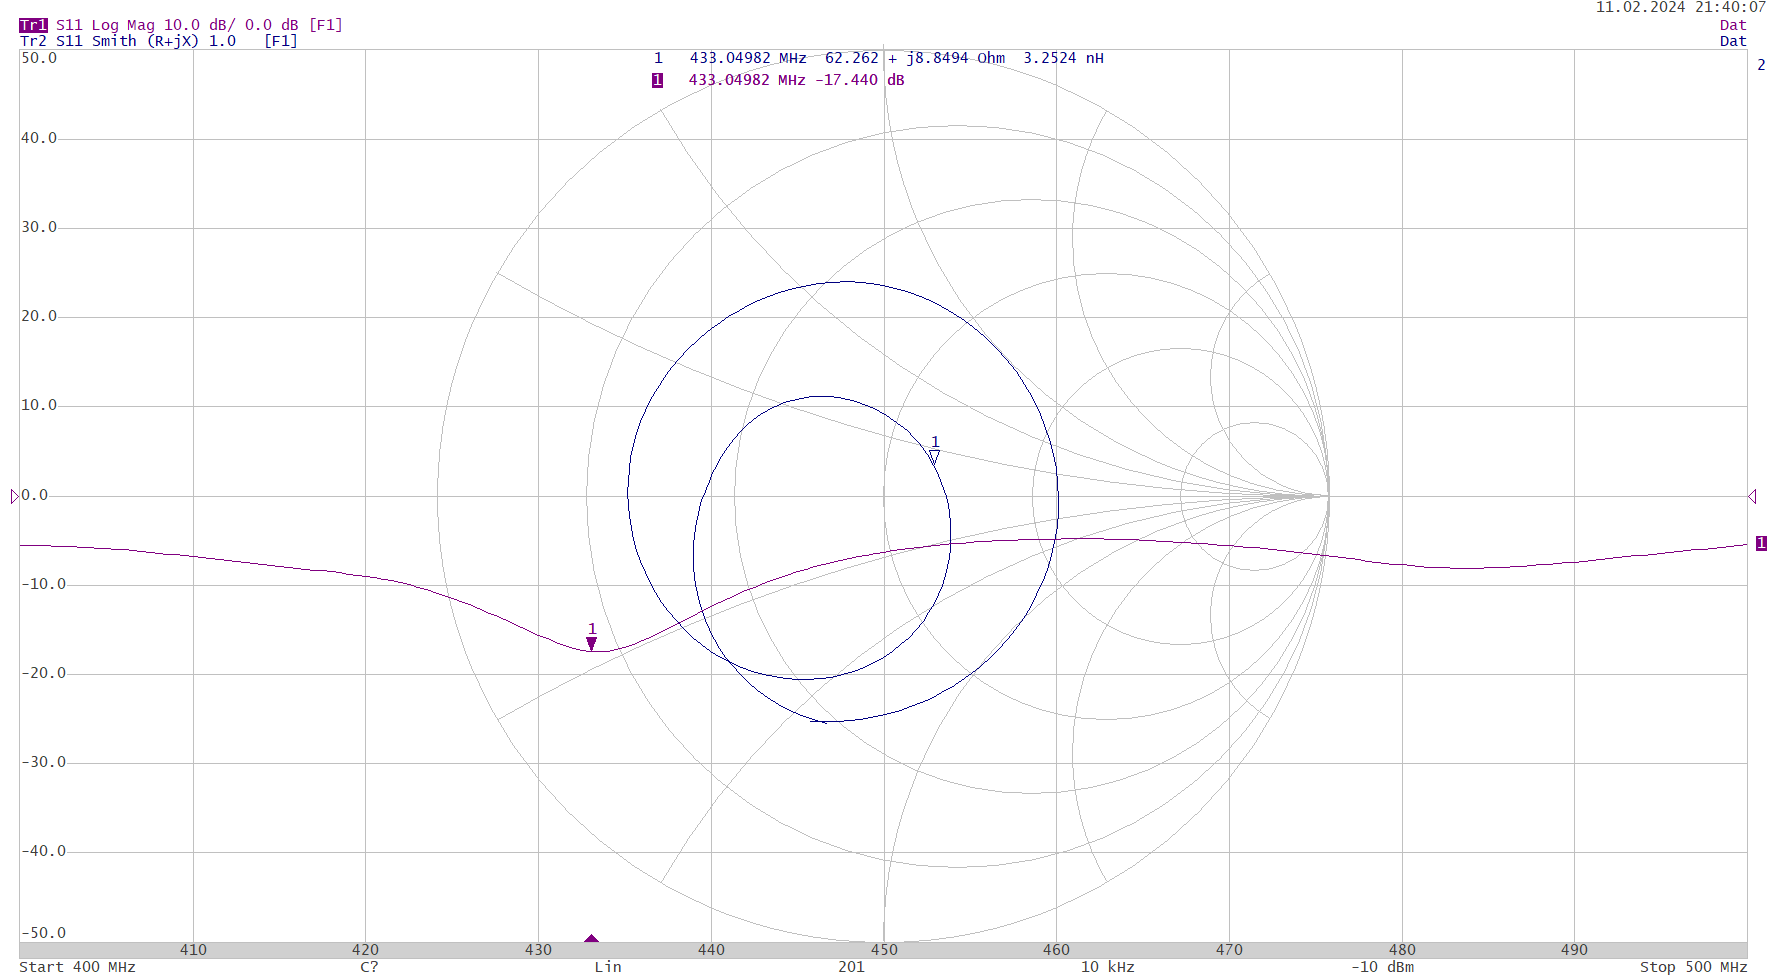
\includegraphics[width=\linewidth]{../ref/qfh_s11.png}
	\caption{S11-Parameter (Rückflussdämpfung) und Smith-Diagramm der fertigen Antenne von 400 bis 500 Megahertz}
	\label{fig:fertig_qha}
\end{figure}

Die Messung zeigt eine maximale Rückflussdämpfung bei fast genau 433 Megahertz. Die Rückflussdämpfung bei 433 Megahertz beträgt -17.44 Dezibel. Für eine minimale Rückflussdämpfung von -10 Dezibel ergibt sich eine Bandbreite von etwa 422 bis 442 Megahertz. Das Smith-Diagramm gibt Aufschluss darüber, dass die Antenne bei 433 Megahertz mit 52.26 Ohm Wirkwiderstand und 8.85 Ohm Blindwiderstand leichte induktive Eigenschaften aufweist.

\subsection{qualitative Charakterisierung}
Zur Charakterisierung der QHA wurde mithilfe eines einfachen Dipols und einem HackRF One als Sender die Antenne aus verschiedenen Richtungen angestrahlt. Mithilfe des SDRs wurde die von der Antenne empfangene Leistung ermittelt. Aufgrund der unbekannten Sendeleistung des HackRF One, welcher nur über eine VGA die bei der Sendefrequenz maximale Sendeleistung kontrolliert, kann keine Aussage über die gesendete Leistung getroffen werden. Dementsprechend beschreiben die nachfolgenden Abstrahldiagramme nur relativ das Abstrahlverhalten der QHA und geben keinen Aufschluss über den wirklichen Gewinn der Antenne. Die dargestellten Werte entsprechen der Differenz der minimal empfangenen Leistung mit -105 dBm und dem Wert der empfangenen Liestung der entsprechenden Ausrichtung. Die Y-Achse entspricht der Vertikalen, die X-Achse der Richtung des Verbindungselements der großen Schleife und die Z-Achse der Richtung des Verbindungselements der kleinen Schleife. Auch die empfangenen Leistungen sollten nur als grobe Messwerte betrachtet werden, da das SDR keinen vollwertigen und kalibrierten Spectrum-Analyzer ersetzen kann. 

\subsubsection{XZ-Strahlungsmuster}
Die nachfolgende Tabelle zeigt die Ergebnisse der Messungen des XZ-Strahlungsmusters, wobei 0 und 180 Grad auf der X-Achse und 90 und 270 Grad auf der Z-Achse.

\begin{tabular}{|c|c|c|}
	\hline
	\textbf{Winkel (in Grad)} & \textbf{Differenz (zu -105 dBm)} & \textbf{Empfangene Leistung (in dBm)} \\
	\hline
	90 & 15,8 & -89,2 \\
	\hline
	45 & 14,2 & -90,8 \\
	\hline
	0 & 14 & -91 \\
	\hline
	315 & 14,9 & -90,1 \\
	\hline
	270 & 16 & -89 \\
	\hline
	225 & 14,5 & -90,5 \\
	\hline
	180 & 15 & -90 \\
	\hline
	135 & 16 & -89 \\
	\hline
\end{tabular}

\begin{figure}[H]
\begin{minipage}[b]{.4\linewidth} % [b] => Ausrichtung an \caption
	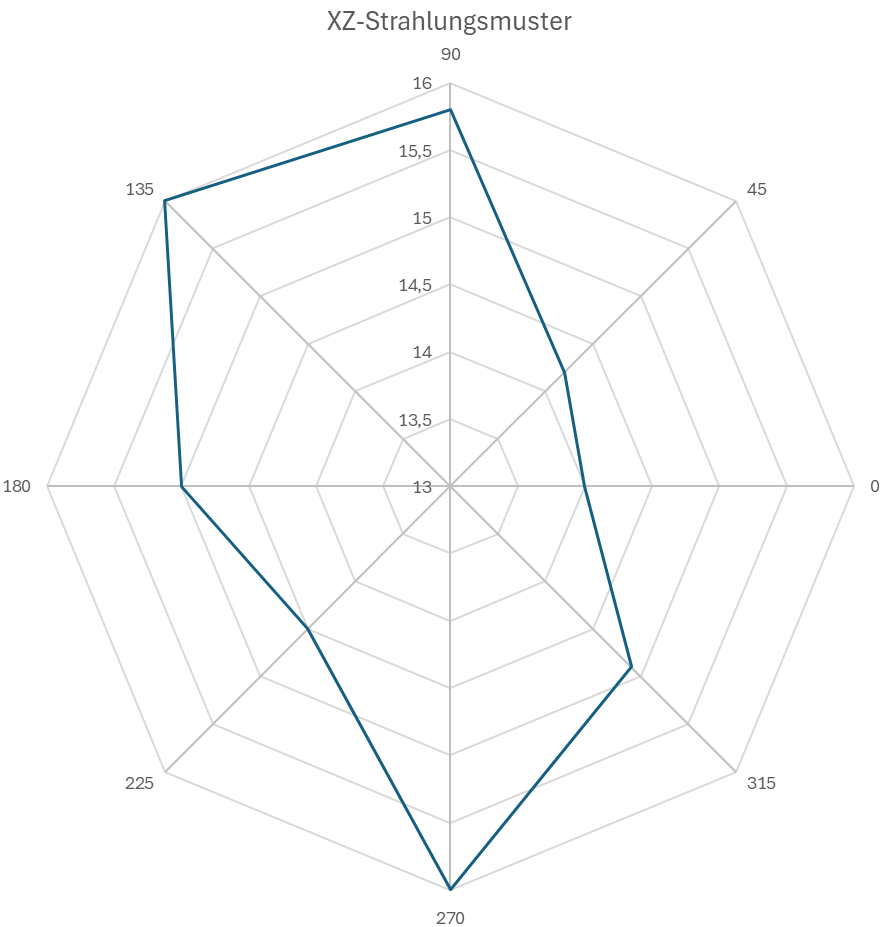
\includegraphics[width=\linewidth]{../ref/XZmeasuredqfh.png}
	\label{fig:XZradiationqfh}
	\caption{qualitatives XZ-Strahlungsmuster der gebauten QHA}
\end{minipage}
\hspace{.1\linewidth}% Abstand zwischen Bilder
\begin{minipage}[b]{.4\linewidth} % [b] => Ausrichtung an \caption
	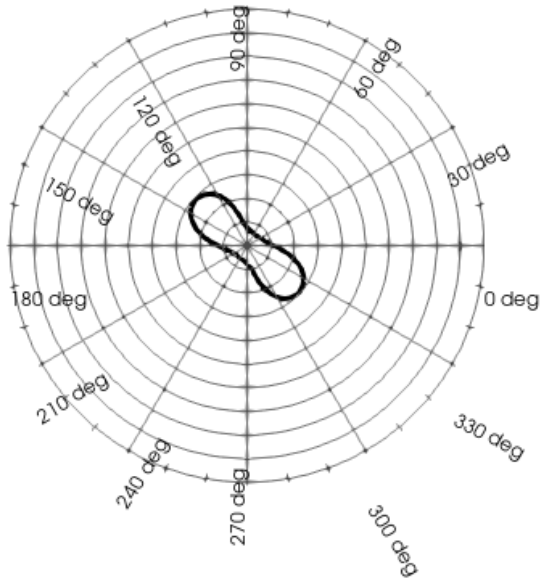
\includegraphics[width=\linewidth]{../ref/XZsimulationqfh.png}
	\label{fig:XZradiationsim}
	\caption{simuliertes XZ-Strahlungsmuster der QHA}
\end{minipage}
\end{figure}

Im direkten Vergleich zwischen dem simulierten und gemessenen Strahlungsmuster ist eine grobe Übereinstimmung der Formen zu erkennen. Auffallend ist vor allem, dass sich das Strahlungsmuster der gebauten QHA um etwa 45° im Uhrzeigersinn verschoben hat. Diese Verschiebung könnte durch Abweichungen von der Simulation zur Realität aber auch durch Messungenauigkeiten begründet sein. 

\subsubsection{YZ-Strahlungsmuster}
Die nachfolgende Tabelle zeigt die Ergebnisse der Messungen des YZ-Strahlungsmusters, wobei der Winkel 90 Grad die Vertikale nach oben beschreibt.

\begin{tabular}{|c|c|c|}
	\hline
	\textbf{Winkel (in Grad)} & \textbf{Differenz (zu -105 dBm)} & \textbf{empfangene Leistung (in dBm)} \\
	\hline
	90 & 15,8 & -89,2 \\
	\hline
	45 & 0 & -105 \\
	\hline
	0 & 17,7 & -87,3 \\
	\hline
	315 & 18,4 & -86,6 \\
	\hline
	270 & 24,7 & -80,3 \\
	\hline
	225 & 18,2 & -86,8 \\
	\hline
	180 & 17,9 & -87,1 \\
	\hline
	135 & 18,7 & -86,3 \\
	\hline
\end{tabular}

\begin{figure}[H]
	\begin{minipage}[b]{.4\linewidth} % [b] => Ausrichtung an \caption
		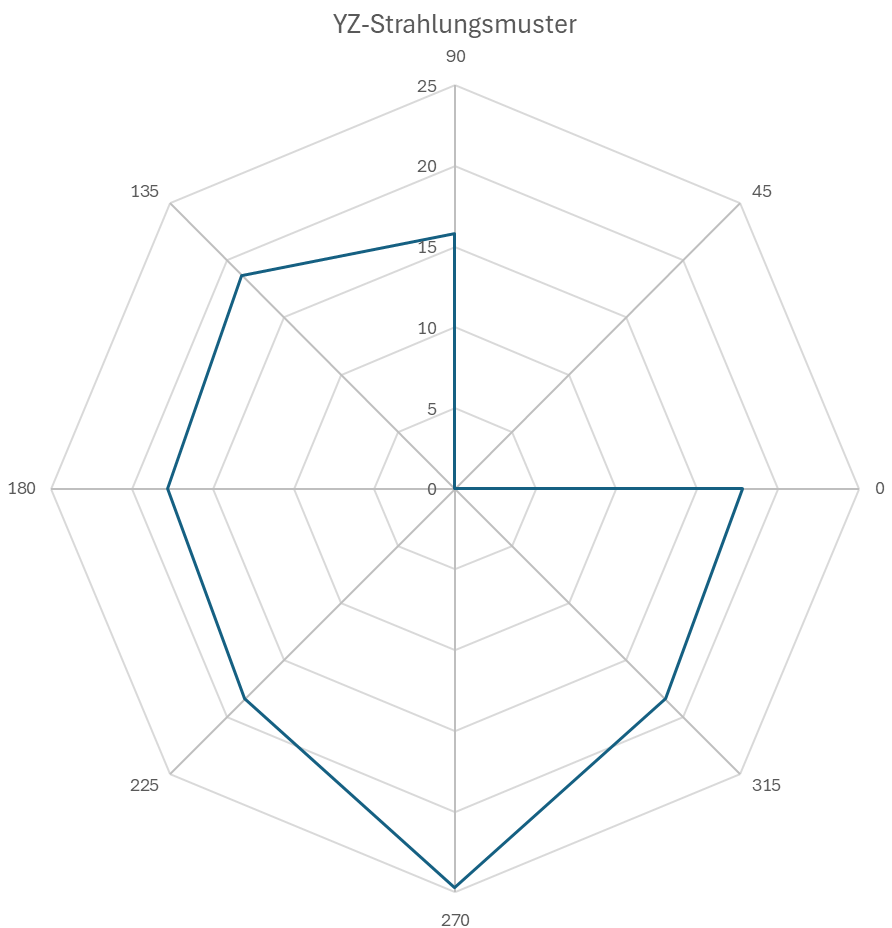
\includegraphics[width=\linewidth]{../ref/YZmeasuredqfh.png}
		\label{fig:YZradiationqfh}
		\caption{qualitatives YZ-Strahlungsmuster der gebauten QHA}
	\end{minipage}
	\hspace{.1\linewidth}% Abstand zwischen Bilder
	\begin{minipage}[b]{.4\linewidth} % [b] => Ausrichtung an \caption
		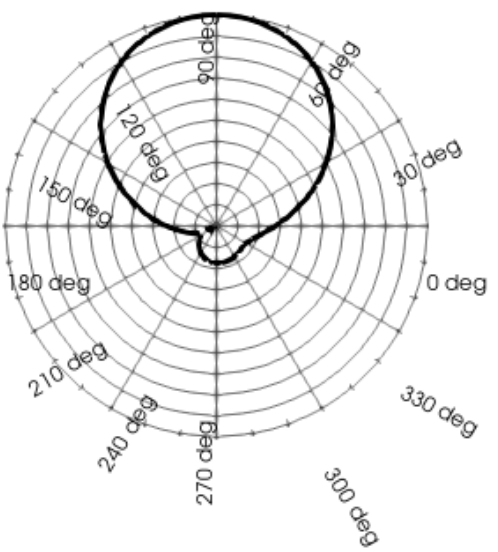
\includegraphics[width=\linewidth]{../ref/YZsimulationqfh.png}
		\label{fig:YZradiationsim}
		\caption{simuliertes YZ-Strahlungsmuster der QHA}
	\end{minipage}
\end{figure}

Deutlich erkennbar bei der Betrachtung des gemessenen Strahlungsmusters ist, dass die QHA, im Vergleich zur Simulation, den besten Gewinn in die um 180 Grad verschobene Richtung, also 270 Grad, aufweist. Wird das simulierte Strahlungsmuster allerdings um 180 Grad gedreht, so sind die Formen nahezu identisch. Auch das Minimum bei etwa 225 Grad in der Simulation ist somit bei 45 Grad in der Messung deutlich zu erkennen. 

\section{Test}
Um die Funktionalität der QHA nachzuweisen wurden mehrere Observationen durchgeführt. Dabei wurde das Signal der QHA zusätzlich mithilfe des im späteren Kapitel \ref{sec:LNA} erläuterten LNA verstärkt. Wichtig zu erwähnen ist, dass die zum Test durchgeführten Messungen vor der Charakterisierung der QHA stattgefunden haben und die Ausrichtung der QHA entsprechend der Simulationsergebnisse vorgenommen wurde. Das trotzdem sehr gute Signale empfangen wurden, könnte durch den dennoch guten Gewinn mit dieser Ausrichtung oder Reflexionen an der Erdoberfläche begründet sein. 

Die Observationen wurden vom 11. bis zum 14. März 2024, an den Koordinaten 47.44983098163626, 9.833138913740827 (Hof 417, 6861 Alberschwende) und auf einer Höhe von 730 Metern über dem Meeresspiegel durchgeführt.  Die Ergebnisse der Observationen, die zum Test der Funktionalität durchgeführt wurden, können unter folgendem Link aufgerufen werden:\newline \url{https://network.satnogs.org/observations/?norad=&start=2024-02-01+17%3A17&end=2024-03-15+17%3A17&observer=&station=3307&transmitter_mode=&transmitter_uuid=&page=1}

\begin{figure} [H]
	\centering
	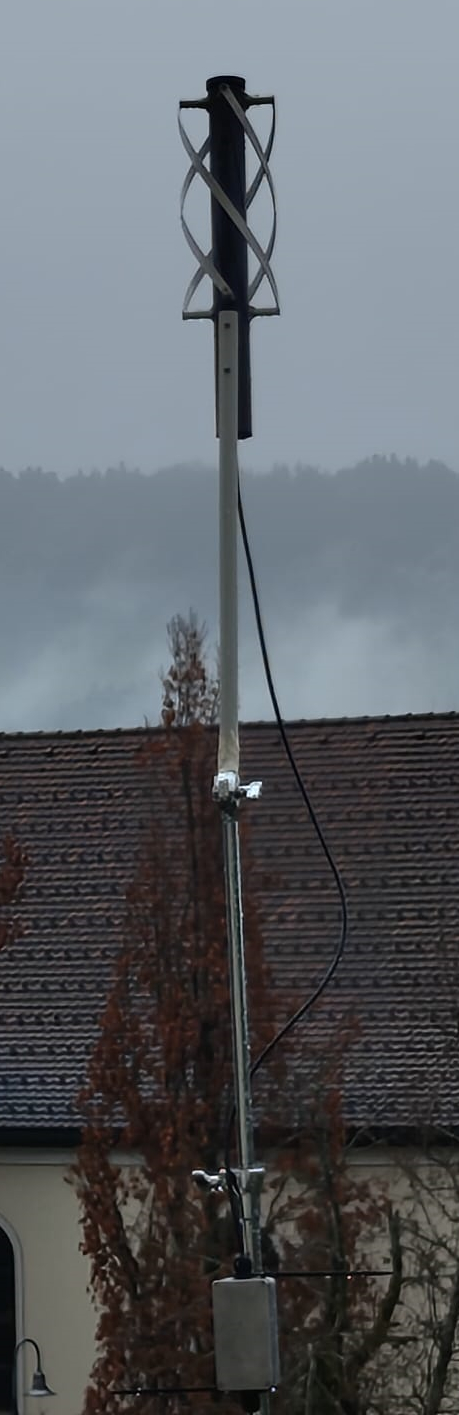
\includegraphics[width=.25\linewidth]{../ref/qha_duringob.jpg}
	\caption{QHA während der Observationen}
	\label{fig:qha_duringobs}
\end{figure}

Mit 45 empfangenen Paketen empfing die Observation mit der Nummer 9196747 des Satelliten \glqq 98959 - SONATE-2\grqq{}  und dem Sender \glqq Mode U - GMSK9k6 - AX.25 G3RUH - Telemetry\grqq{} die meisten Datenpakete. Die Daten wurden am 14. März 2024 von 00:16:04 bis 00:23:36 (UTC) empfangen. Die nachfolgende Abbildung zeigt das Wasserfalldiagramm sowie das erste dekodierte Datenpaket im HEX und AX.25 Format.

\begin{figure} [H]
	\centering
	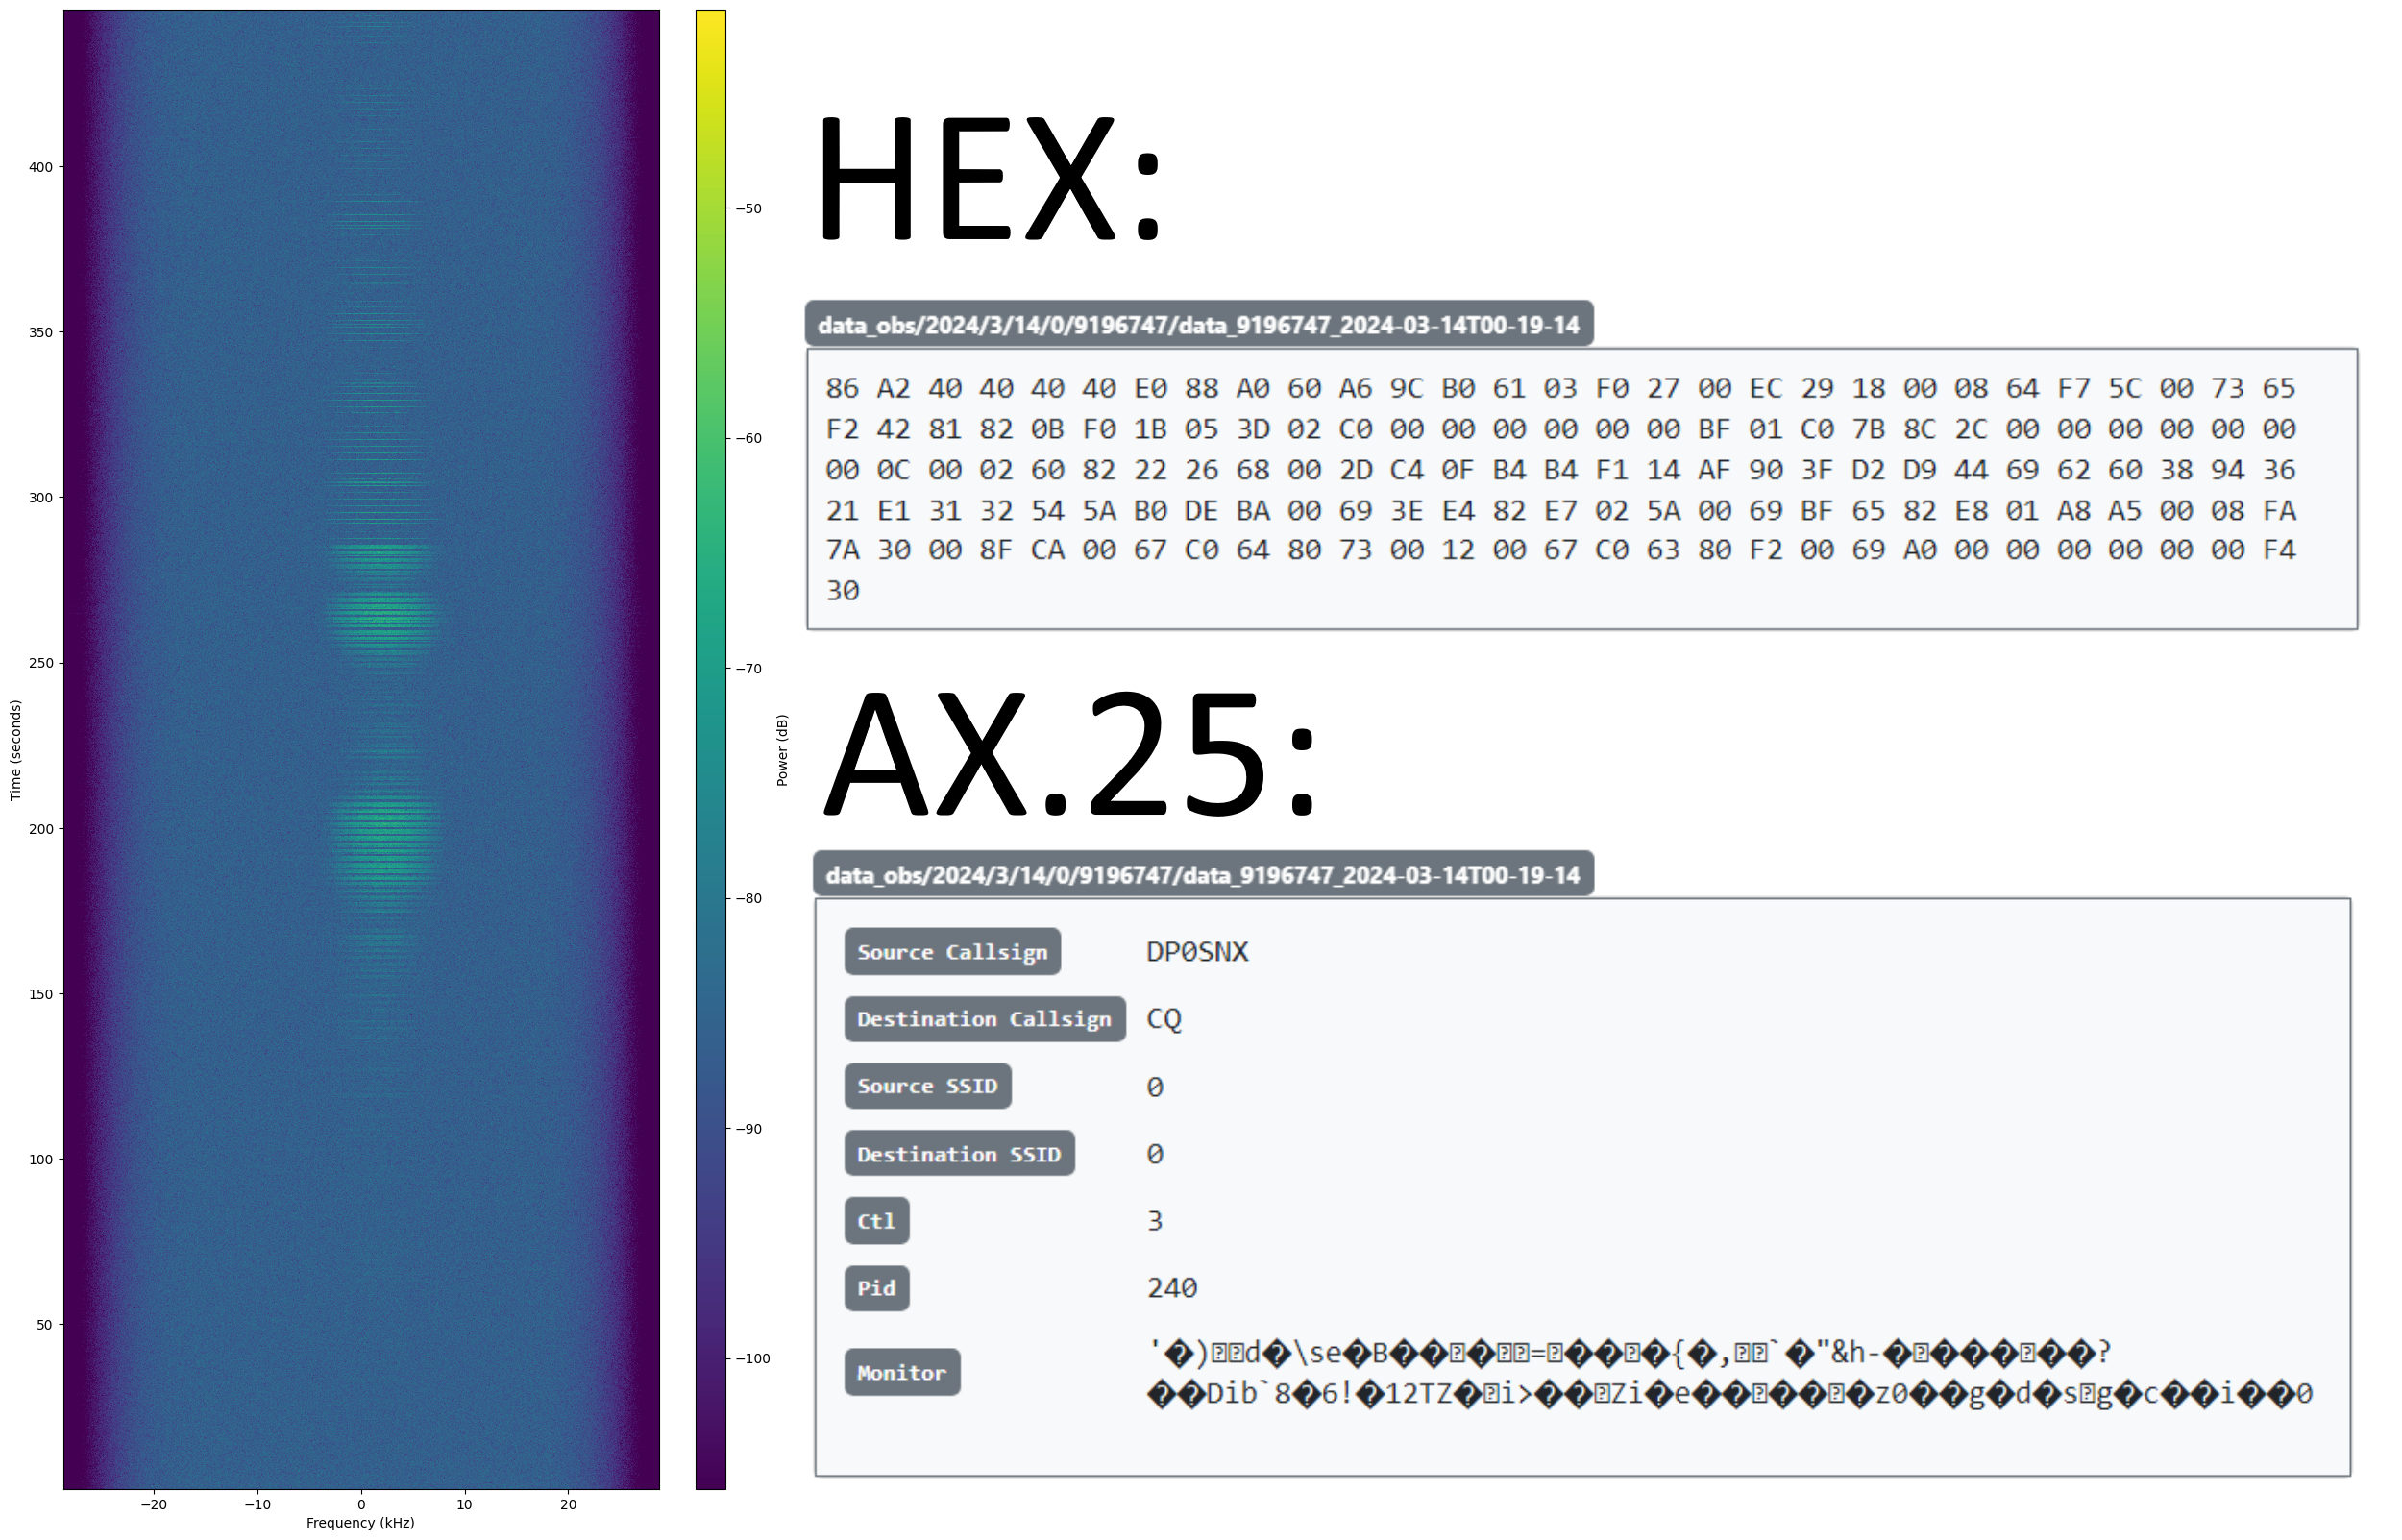
\includegraphics[width=\linewidth]{../ref/qha_successfull_operation.png}
	\caption{Wasserfalldiagramm und erstes Datenpaket in HEX und AX.25 Format der Observation 9196747 \cite{noauthor_satnogs_qfh_observation_nodate}}
	\label{fig:qha_successfull_observation}
\end{figure}